\section{Framework and API}
Given a dataset with a mix of ``interpretable'' (structured features) and ``uninterpretable'' (unstructured / high-dimensional features), \sys uses an EM-like algorithm to learn a set of rules over the interpretable features that partition the predictive behavior of the model.
These partitions can be used to isolate subsets of training data that affect the prediction of a new test example.

\subsection{Notation}
Let the training dataset $D$ contain tuples of features $x_i$ and labels $y_i$ that are categorical or real-valued.
\texttt{train(D)} is a training algorithm that returns a model \texttt{model($\cdot$)} that takes as input a test point $x_{new}$ and predicts a label $\hat{y}_{new}$:
\[
\hat{y}_{new} = \textsf{model}(x_{new})
\]

Consider the following running example of car insurance fraud detection. The training dataset $D$ has the following schema:
\[
\texttt{D(make, amount, at\_fault, descr, fraud?)}
\]
where \texttt{make} is a categorical attribute describing the make of the car, \texttt{amount} is a double-valued amount that the person is claiming, \texttt{at\_fault} is a boolean variable describing whether the claimant is at fault, \texttt{descr} is a string-valued attribute describing the nature of the claim, and \texttt{fraud?} is the yes/no label if the claim is fraudulent.

Suppose $\textsf{model}(\cdot)$ issues an incorrect prediction and erroneously flags a fraudulent claim as not fraudulent. The data scientist is now tasked with debugging the model to understand why this error happened. 
If she was using a simple model, like a decision tree, she might be able to look at the structure of the model and determine whether it matches intuition (e.g., fraudulent claimants tend not to claim they were at fault).
However, sometimes the prediction problem necessarily needs a more complex learning model. For example, there is a textual field \textsf{descr}, which might be a very valuable feature for predicting fraud. Processing such data typically requires translating the data into a higher-dimensional feature space by using NLP methods such as word-embeddings, stop word removal, bi-gram featurization, etc.  By design, this feature space may not be interpretable by anyone other than a language expert, and using a simpler model may not achieve the desired accuracy. Furthermore, highly expressive deep models such as deep neural networks, which in principle can learn any deterministic function, are susceptible to adversarial examples (i.e., imperceptible perturbations to the features that cause a change in prediction)\cite{szegedy2013intriguing}. 
This means that relying on neighboring points can be unreliable or even misleading because they may inadvertently be adversarial.  

\subsection{Debugging with \sys}
The approach that we propose identifies records that the {\it classifier} considers similar, rather than naive similarity in the feature space.
As an illustrative example, imagine if we hard-coded the following logic:
\begin{lstlisting}
def smodel(x):
    if amount > 10000:
    #one model for larger claims
        return submodel_1(x)
    elif a_fault:
    #one model for small at fault claims
        return submodel_2(x)
    else:
    #a default model
        return submodel_3(x)
\end{lstlisting}
In this function, interpretable rules assign new data to submodels (which encapsulate the complexity).
Although the rules are simple, the full function \texttt{smodel} can still model complex patterns due to the complex sub-models.
If we observe an anomaly, the developer can precisely blame one of the submodels; thereby, providing a coarse predicate to select tuples that are assigned to that model.
Furthermore, the rules illustrate the implicit partitions and decision structure of the function.

Given this intuition, \sys explores whether we can synthesize such code structure automatically to mimic black-box (but differentiable) models.
An interpretable meta-model over the structured features (e.g., make, amount, at\_fault), assigns a test example to a more complex sub-model over all features.
The interpretable meta-model is represented as a decision tree (if-else statements), and the sub-model is allowed to be of the same class as the original model.
In the inference procedure, we learn the most likely decision tree over the interpretable features a set of sub-models that explain a models predictions.
There is an inherent tradeoff, a meta-model that contains a single partition \texttt{true} can create a sub-model that is nearly identical to the original complex model. However the partition is not useful to the developer.  In contrast, increasing the complexity of the meta-model makes each partition smaller, but the resulting model potentially diverges from the original model.  At the limit, the meta-model may simply build a decision tree over the training data, and each partition contains nearly identical points.
We present initial results exploring these tradeoffs in the experiments.

The inference algorithm can run offline during the training phase and is no-more than a constant factor more expensive than standard model training
We presented a generalization in prior work~\cite{DBLP:journals/corr/KrishnanGLMPG16, krishnan17}. 
At a high-level, the algorithm takes the dataset $D$ and the model \textsf{model} as input, and returns $\textsf{smodel}$, which consists of a decision-tree meta model that selects from a collection of $k$ submodels. Given a new record, the user can evaluate both:
\[
\hat{y}_{new} = \textsf{model}(x_{new})
\]
\[
\hat{y}_{new} = \textsf{smodel}(x_{new}) \approx \textsf{model}(x_{new})
\]
and use the structure of \textsf{smodel} to debug with knowledge that it approximates $\textsf{model}$.

\subsection{API and System}
Our current implementation is in Python and focused on TensorFlow models.  The user supplies:
\begin{itemize}
\item \emph{Featurized Dataset. } The user provides a dataset of feature and label tuples.

\item \emph{Explainable Features. } The user lists a subset of features that are understandable.

\item \emph{Tensorflow Model Description. } The user provides a symbolic description of the model in Tensorflow.

\item \emph{Number of Sub-models. } The user provides the number of submodels to include in the surrogate model (denoted as $k$).
\end{itemize}

The output of the system is:
\begin{itemize}
\item \emph{Original Model. } The original model trained to completion

\item \emph{K Sub-Models. } The system returns K submodels trained on different partitions of the feature-space.

\item \emph{Decision Tree Meta Model. } The system returns a meta model that switches between the K submodels based on the input record.
\end{itemize}

\iffalse
We implemented the algorithm into a web interface that allows users to debug TensorFlow models Figure \ref{fig:interface}. The interface shows users mispredictions and allows them to search records that the classifier treats as similar.

\begin{figure*}[t]
    \centering
    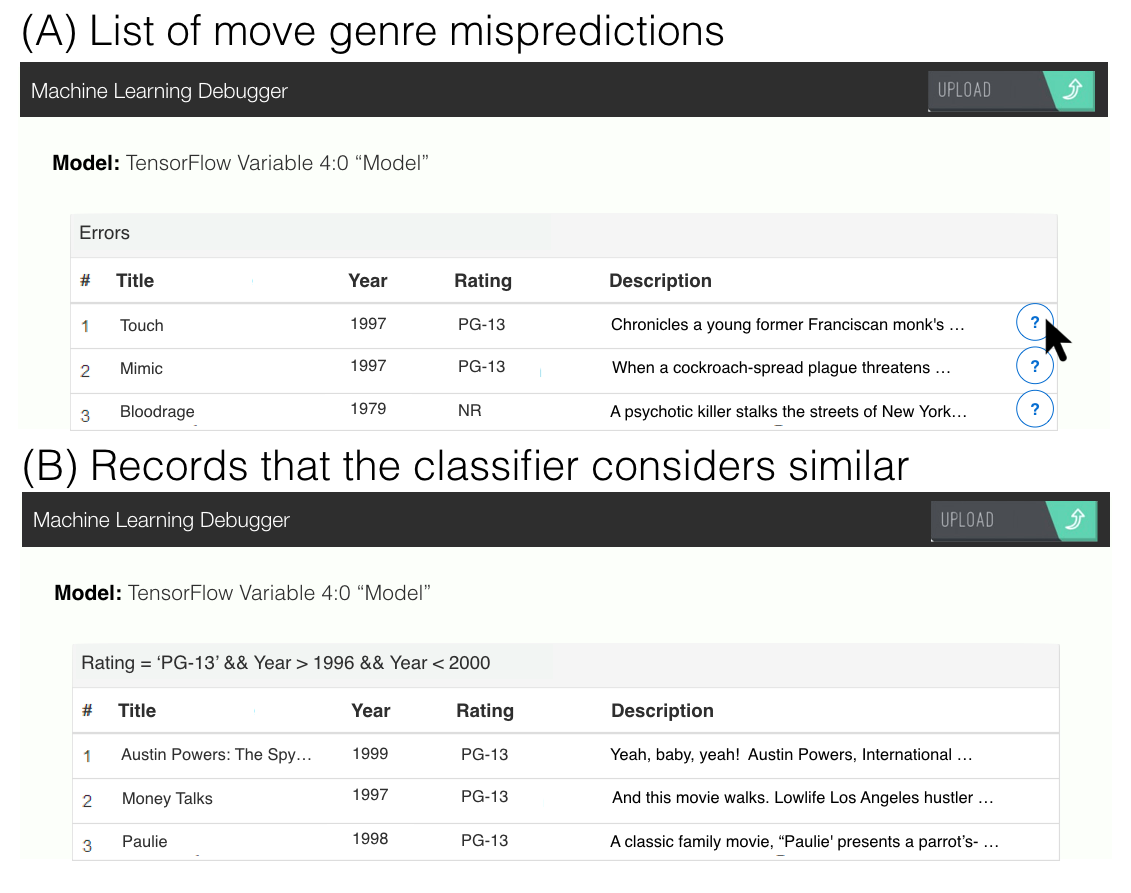
\includegraphics[width=0.5\textwidth]{figures/interface.png}
    \caption{A prototype interface implementing the algorithm. In (A), the interface lists a set tuples that were mis-predicted. Users can dig deeper by selecting one such tuple. (B) is the following panel which describes a predicate and records that the classifier considers as similar.}
    \label{fig:interface}
\end{figure*}
\fi